\documentclass[12pt,twoside]{report}
\usepackage[utf8]{inputenc}
\usepackage{graphicx}
\usepackage{float}
\usepackage{authblk}
\graphicspath{ {images/} }

\usepackage[
backend=biber,
style=numeric,
sorting=none
]{biblatex}

\addbibresource{SIPref.bib}

\usepackage[a4paper,width=150mm,top=25mm,bottom=25mm,bindingoffset=6mm]{geometry}

\usepackage{fancyhdr}
\pagestyle{fancy}
\renewcommand{\chaptermark}[1]{\markboth{\MakeUppercase{#1}}{}}
%\fancyfoot{}
%\fancyfoot[LE,RO]{\thepage}

\begin{document}
\begin{titlepage}
    \begin{center}
        \vspace*{1cm}
        
        \Huge
        \textbf{Cavitation of Electron Bubbles In Liquid Helium-4}
        
        \vspace{0.5cm}
        \LARGE
        %Thesis Subtitle
        
        \vspace{1.5cm}
        
        \textbf{Kevin H. Bhimani}\footnote{Department of Physics, Kalamazoo College, Kalamazoo, MI}\\
        Supervisor: Dr. Jan Tobochnik$^1$\\
        In collaboration with: Dr. Humphrey Maris\footnote{Department of Physics, Brown University, Providence, RI} and Dr. Yiming Yang$^2$
        \vfill
        
       Thesis submitted in partial fulfillment of the requirements for the degree of Bachelor of Arts.
        \vspace{0.8cm}
        
        
\includegraphics[height=0.2\textwidth]{Klogo.jpg}
        
        \Large
        Kalamazoo, Michigan\\
        September 2018
        
    \end{center}
\end{titlepage}

\chapter*{Abstract}
Electron bubbles in liquid helium form an interesting quantum mechanical system. The electron bubbles can be cavitated by introducing a critical negative pressure in the form of sound waves. Experiments suggest that there are two such critical pressures: each one occurring with a different mechanism. We study the relationship of this critical pressure with variation in temperature, static pressure, and frequency of the sound. Experimental data also suggest the existence of a new event called a very rare event of which not much is known. Below a certain temperature, the value of the critical pressure deviated from theoretical predictions. We performed calculations for nonlinear propagation of sound to explain these deviations. The simulations successfully modeled the system and it was concluded that the propagation of sound in liquid helium is nonlinear.

\chapter*{Acknowledgements}
 This work is based on the research I did in the electron bubble group at Brown University during summer of 2017. I want to thank Dr. Humphrey Maris for having me work in his lab for the past two summers. I value deeply all the advice and assistance he has provided. I would also like to thank Dr. Yiming Yang for explaining to me the experiment in detail, always answering my questions, and providing plots from his thesis.

I am grateful to Dr. Jan Tobochnik for being my undergraduate mentor and for providing feedback, support and advice during the entire project. Finally I would like to thank Jessica Wile for proof reading this thesis. This work was funded by Kalamazoo College's Center for Career and Professional Development and Sherman Fairchild Foundation.

\tableofcontents

\chapter{Introduction}
An electron bubble is a stable configuration that a free electron acquires in liquid helium. \cite{Classen} The electron is repelled by a helium atom because if it tries to pass through the atom, it has to go into a n=2 state. This makes the energy of the electron about 1 eV higher than the energy in the vacuum. But, it turns out that, the electron can lower its energy by creating a bubble in the liquid that is free of helium atoms. The electron losses its energy either by scattering helium atoms, by ionizing helium atoms, or by exciting the atoms. The formation of the electron bubble is demonstrated in Fig. \ref{bubbleFormation}.
\begin{figure}[H]
\centering 
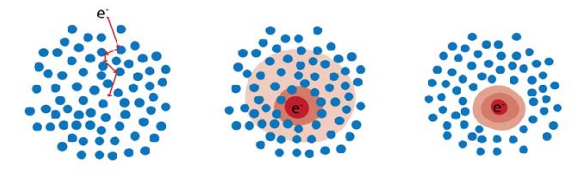
\includegraphics[width=100mm, height=30mm]{Introduction/bubbleFormation.png}
\caption{Process for formation of electron bubbles. \cite{Yang2018thesis}}
\label{bubbleFormation}
\end{figure}

The energy of this bubble can be be approximated as follows:
\begin{equation}\label{energyEqbub}
E=\frac{h^2}{8mR^2}+4\pi R^2\alpha + \frac{4}{3}\pi R^3 P
\end{equation}
where $\alpha$ is surface tension, $R$ is the radius of the bubble, $h$ is Plank's constant, $m$ is the mass of an electron, and $P$ is the applied pressure. Equation \ref{energyEqbub} can be understood as the sum of zero-point energy of the electron (the energy of electron due to being confined in a potential well that is the bubble), the surface energy of the bubble, and the volume energy of the bubble: the work done while creating the bubble over pressure $P$.  

If we assume that $P=0$, differentiating Eq. \ref{energyEqbub} and setting it to zero, the energy has a minimum at
\begin{equation}\label{minEnergy}
R_{min} = \left(\frac{h^2}{32\pi m \alpha}\right)^{1/4}
\end{equation} 
From Eq. the \ref{minEnergy}, value of $R_{min}$ is $19 \AA$ at $0K$. This gives a good intuition of how big electron bubbles are. These bubbles are subjects of ongoing research and have led to many surprising results. 

In one such experiment, electron bubbles were subjected to an applied electric field. \cite{Wei2016} The goal was to determine the mobility of electron bubbles in superfluid helium where the mobility is restricted mainly by thermal excitation: phonons and rotons (explained in detail in Chapter 2). In this experiment, electron bubbles were introduced at the top of a cell containing liquid and the time it takes for them to reach the bottom positive plate was recorded. They were expected to reach the bottom plate about the same time since electron bubbles all have the same mobility. Thus it was expected that there would be a sharp decline in voltage when these electron bubbles reached the bottom plate. This voltage change was indeed observed, but as the Fig. \ref{exo_ions} shows there were other bubbles which traveled faster than ordinary electron bubbles and arrive quicker.  
\begin{figure}[H]
\centering 
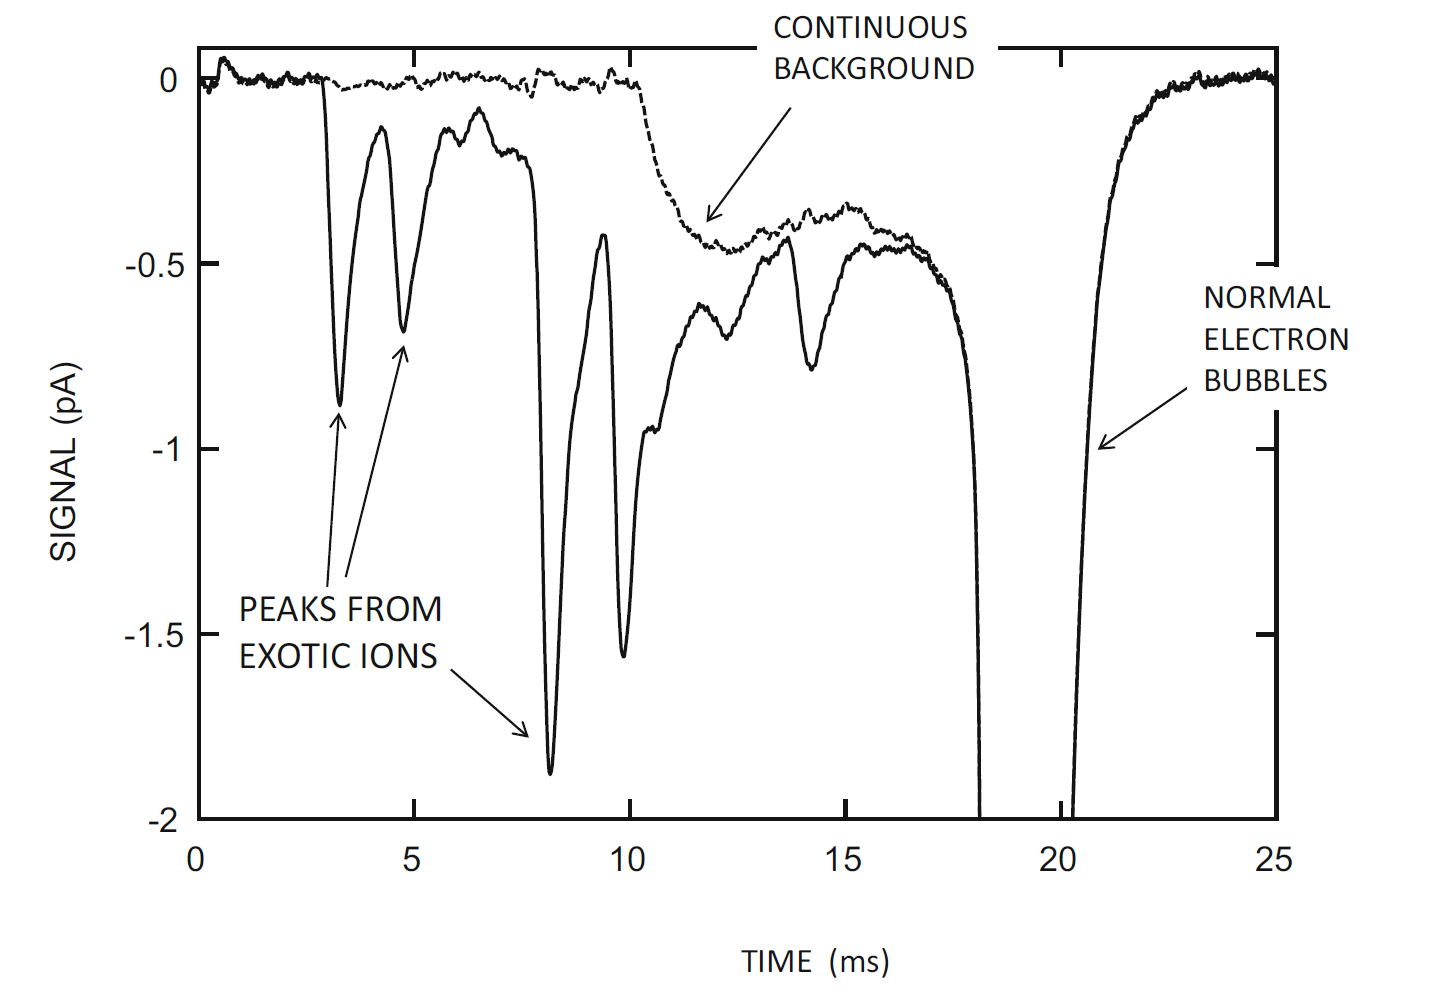
\includegraphics[width=110mm, height=80mm]{Introduction/exo_ions.png}
\caption{Solid curve showing the current arriving at the collector as a function of time. \cite{Wei2016}}
\label{exo_ions}
\end{figure}

The first ion to reach the detector was termed fast ion and was first observed by Doake and Gribbon. Shortly after the discovery of the fast ion, Ihas and Sanders discovered several other ions having mobility between the fast ion and the electron bubble. To this date, at least 18 such ions have been observed. A continuous background is also observed. This background is quite surprising since it implies that there are ions that have a continuous distribution of size. These bubbles are called the exotic ions and appear to be smaller than ordinary electron bubbles.

There is no general explanation for the existence of exotic ions. One might consider that they are impurities in liquid helium; however, that would imply that there are 18 different impurities in liquid helium. This is not probable since the number density of impurities in liquid helium is expected to be very small. Another possible explanation is that the exotic ions are negatively charged helium atoms. While it is true that ions of both helium atoms and helium dimers have been observed, they cannot explain the continuous background. Moreover, their lifetime is quite short. Therefore, it is unlikely that they pass through the mobility cell in the experiments-- where the time has been as large as $100 ms$.

Considering the bubble as a Quantum Mechanical system might provide a solution. The proposed fission model suggests that the exotic ions are bubbles that contain a fraction of the total wave function of an electron. If a fraction of the wave function, $\psi$, is in a bubble, then the bubble would be smaller in size than an electron bubble. The integral of $|\psi^2|$ over the bubble could have a continuous range of values and that could potentially explain the continuous background. A detailed mathematical analysis can be found in \cite{Wei2016}.

A further investigation is needed in order to understand the structure and origin of exotic ions. However, much simpler experiments need to be performed on electron bubbles before designing experiments for exotic ions. This is because electron bubbles are relatively well understood and have been studied for a long time. This thesis reports one such experiment.

Our experiment involved studying the effects of sound waves on electrons bubbles. This was done by introducing a negative pressure to an electron bubble at the focus of a piezoelectric transducer. The critical pressure at which an electron bubble bursts was studied against temperature, static pressure and frequency of sound.

\chapter{Nucleation Experiment}
\section{Superfluidity in liquid helium}
Liquid helium has been found to be an useful liquid to study macroscopic quantum phenomena. This is because helium has a remarkable property of exhibiting superfluidity below $2.17$ K at a pressure of $1$ atm. The temperature of $2.17$ K is commonly known as the Lambda point. Below the Lambda point the behavior of liquid helium is explained by the two-fluid model. According to this model liquid helium has two components, normal fluid component with density $\rho_n$ and superfluid component with density $\rho_s$. 

The phase diagram for helium is shown in Fig. \ref{phaseDiaHe}. The diagram shows that helium is liquid under a broad range of pressure at $0$ K. This fact does not violate the Third law of Thermodynamics since all atoms are in the same quantum state and thus identical. This will make the entropy zero. At $0$ K the entire liquid is superfluid. 
\begin{figure}[H]
\centering 
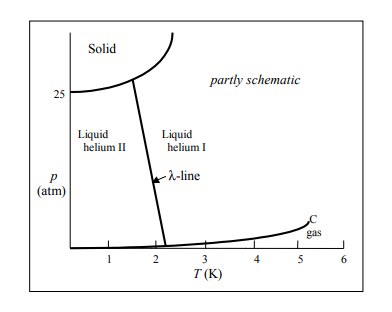
\includegraphics[width=90mm, height=70mm]{Nucleation_Experiment/He_phaseDiagram.png}
\caption{Phase Diagram for $^4He$. \cite{Vinen:808382}}
\label{phaseDiaHe}
\end{figure}

Elementary excitations in liquid helium below the lambda point are in the form of phonons and rotons. These excitations can be explained by studying the plot of energy vs momentum of $^4He$ as shown in Fig. \ref{elementaryExcitation}. This relation is linear at first. Excitations in this region are called phonons and these are high frequency sound waves. The plot has a minimum in energy. The excitations in this region are called rotons and these are excitations with very short wavelengths. Rotons are the ones that make bigger contribution to the specific heat and the thermal energy of Helium at $1$ K and above.
\begin{figure}[H]
\centering 
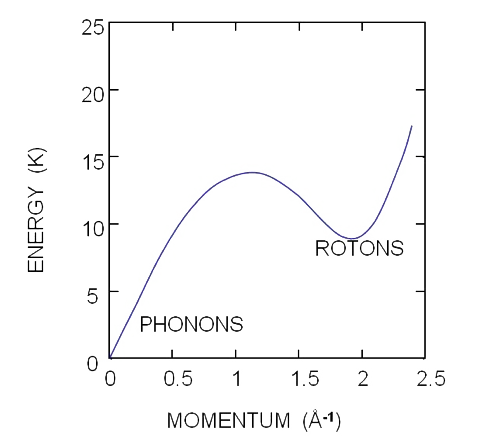
\includegraphics[width=100mm, height=80mm]{Nucleation_Experiment/elementaryexcitations.png}
\caption{Energy versus Momentum for $^4He$. \cite{rotonFig}}
\label{elementaryExcitation}
\end{figure}

Thus helium has a very well studied excitation structure. This fact makes it an ideal liquid to experiment with electron bubbles and study exotic ions. Below the liquid-gas co-existence line, a given state- solid or liquid- can be kept as a metastable state and a phase transition can be introduced only when an energy barrier is overcome. A large nucleus is formed and such a formation is termed homogeneous nucleation. A similar nucleation can be formed at an interface of the helium and impurities, called heterogeneous nucleation.

\section{Nucleation theory}
Nucleation is a general concept that means formation of phase or structure in a homogeneous medium. Cavitation means the nucleation of vapor bubbles in a liquid. To understand cavitation, consider a free vapor bubble in a bulk liquid. The energy required to create such a bubble can be written as the sum of the surface energy of the bubble and the volume energy of the bubble as shown in Eq.\ref{homoBubbleenergyEq}.
\begin{equation}\label{homoBubbleenergyEq}
\Delta E = 4\pi R^2\alpha + \frac{4}{3}\pi R^3\Delta P
\end{equation}
$\alpha$ is the surface tension and $\Delta P = P_{svp} - P_x$ where $P_{svp}$ is the saturated vapor pressure and $P_x$ is the new pressure. A plot of this energy versus radius is shown in Fig. \ref{energyBarrier}.
\begin{figure}[H]
\centering 
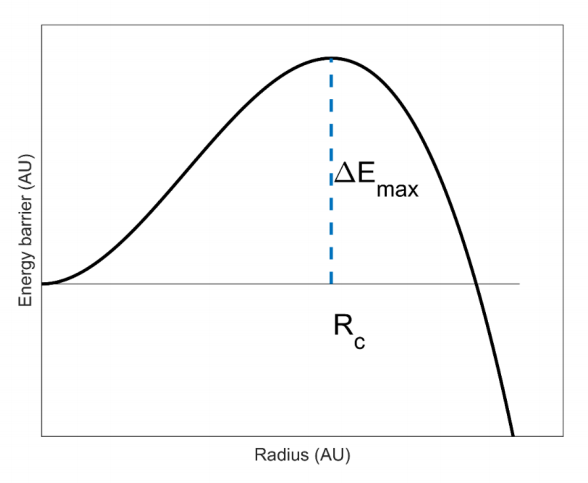
\includegraphics[width=100mm, height=80mm]{Nucleation_Experiment/energyBarrier.png}
\caption{Energy versus Pressure for a gas bubble. \cite{Yang2018thesis}}
\label{energyBarrier}
\end{figure}

Classically, one can obtain the critical radius by differentiating $\Delta E$ with respect to $R$ and setting that to zero. It turns out that
\begin{equation}\label{critRadius}
R_c = \frac{2\alpha}{|\Delta P|}
\end{equation}
Incorporating Eq. \ref{critRadius} into Eq. \ref{homoBubbleenergyEq} we get the energy barrier $\Delta E_{max}$
\begin{equation}\label{energyBarriereq}
\Delta E_{max} = \frac{16\pi \alpha^3}{3|\Delta P|^2}
\end{equation}
Thus a bubble with a radius greater than $R_c$ would grow to a macroscopic size since that is energy favorable. A bubble can be made to reach this critical radius by applying negative pressure by the means of sound waves.

The same calculation can be applied to electron bubbles where the energy is given as:
\begin{equation}\label{energyEq}
E=\frac{h^2}{8mR^2}+4\pi R^2\alpha + \frac{4}{3}\pi R^3 (P-P_{svp})
\end{equation}
The energy versus radius is plotted in Fig. \ref{bubble_energyBarrier} for different values of $\Delta P$.
\begin{figure}[H]
\centering 
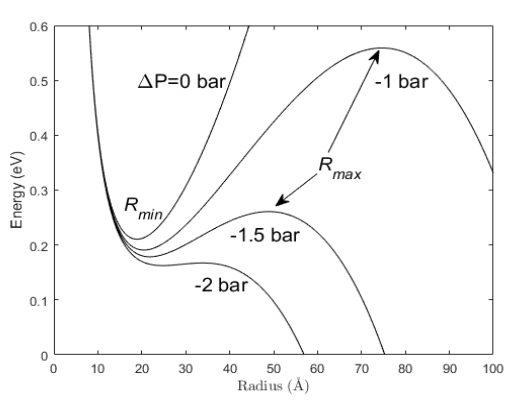
\includegraphics[width=100mm, height=80mm]{Nucleation_Experiment/bubble_energyBarrier.png}
\caption{Energy versus Pressure for an electron bubble. \cite{Yang2018thesis}}
\label{bubble_energyBarrier}
\end{figure}
It is evident that an energy barrier does exist, but only for negative values of $\Delta P$. Otherwise, the electron bubble is stable. Therefore a negative $\Delta P$ is needed in order to nucleate an electron bubble.
Setting $\left.\frac{dE}{dR}\right|_{R_c} = 0$ and $\left.\frac{d^2E}{dR^2}\right|_{R_c} = 0$ we get
\begin{equation}\label{critPresseq}
P_c=-\frac{16}{5}\left(\frac{2\pi m}{5h^2}\right)^{1/4}\alpha^{5/4}
\end{equation}
and
\begin{equation}\label{critRadeq}
R_c = \left(\frac{5h^2}{32\pi m\alpha}\right)^{1/4}
\end{equation}
The experiment is used to verify that the critical pressure agrees with the theoretical formula given by Eq. \ref{critPresseq}. Then the same experiment can be performed to find the critical radius and critical pressure for exotic ions where there is no theoretical prediction.

\section{Heterogeneous nucleation}
There are at least three types of heterogeneous nucleation. The first type being from normal electron bubbles produced by introducing a radioactive beta source. The electrons from the source can also excite helium atoms and cause the second kind of heterogeneous nucleation. In this process, the excited helium atoms get ionized and the resultant electron is called a secondary electron. This electron would be quickly pulled backed to the positive ion due to electrostatic force; however, before recombination the electron can form a bubble and be cavitated. The third one is due to a process called Penning ionization. After the recombination, a helium atom is in an excited state and will combine with another helium atom in the ground state to form a dimer.
$$He^*+He\rightarrow He^*_2$$
Then by Penning ionization process, two dimers can be annihilated.
\begin{equation}\label{HeliumEq1}
He^*_2+He^*_2 \rightarrow 3He +He^+ + e^-
\end{equation}
or
\begin{equation}\label{HeliumEq2}
He^*_2+He^*_2 \rightarrow 2He + He^+_2 + e^-
\end{equation}
Thus in principle, there should be two different thresholds for cavitation by electrons. The first one due to electrons coming from the beta source. The second one is due to secondary electrons and electrons due to the Penning ionization process. Classen et al \cite{Classen} reported two different thresholds for cavitation by electrons when they conducted experiments with a thallium source. They reported two different critical pressures at which the nucleations were observed. The first one $|P_{rare}|$ was due to electrons from the source and the second was due to the secondary electrons $|P_{secondary}|$. There was a third new critical pressure between these pressures. The events due to this were termed rare events since the probability of them was very low. Our experiments suggest that $|P_{secondary}| = |P_{dimers}|$.
\section{Experimental setup}
The cryostat structure is shown in Fig. \ref{cryostatfig}. The bubbles are nucleated in a piezoelectric transducer located inside the cell. There are several baths to cool the cryostat. Liquid nitrogen baths are located towards the outside and have their own pumping lines. The helium baths are on the top and are filled with liquid helium. In order to have extreme purity inside the cell, ultra pure helium gas is liquidized using the helium baths. This cooling power comes from the evaporation of liquid in the helium baths. Then the top of each helium bath is pumped. The evaporating helium from the baths will absorb heat from the pumping lines that contain the ultra pure gas. Ultimately, this gas would liquidify and fill the cell. 

While using $^4He$, temperatures as low as $1$ K can be reached by using this process. The second pot is used to provide thermal anchoring for the main pot. There was a radioactive $\beta$ source on top of the transducer that introduced electrons to the cell. In order to study homogeneous nucleation, a potential is applied between the transducer and the source. If $\Delta$V is negative, the electrons would not arrive at the transducer and the nucleation would then be because of secondary electrons and as a result of the Penning ionization process.
\begin{figure}[H]
\centering 
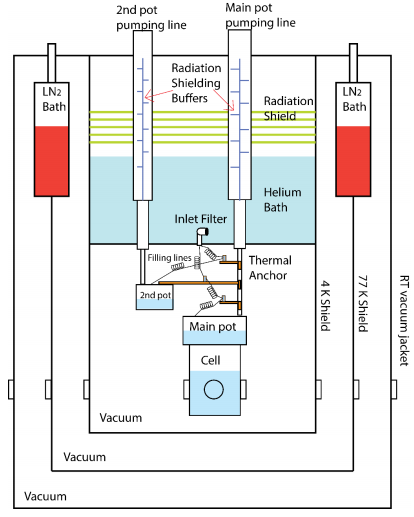
\includegraphics[width=90mm, height=120mm]{Nucleation_Experiment/cryostat.png}
\caption{Design of the cryostat. \cite{Yang2018thesis}}
\label{cryostatfig}
\end{figure}
The transducer had an outer diameter of $2.54$ cm and a thickness of $0.49$ cm. It had two resonance frequencies at $115$ kHz and $471$ kHz. When the transducer is operated at $115$ kHz, it is said to be operated on a flexural mode, and when it is operated at $471$ kHz, it is said to be operated on a thickness mode. The names come from the fact that the transducer vibrates with different mechanisms at each of the two frequencies. 

The sound waves produced by the transducer would collect at the focus and that is where the nucleation is observed. The focus is targeted by a laser beam of wavelength $532$ nm and a power of about $30$ mW. A lens is used to converge the laser at the focus. 

If an electron bubble were present at the focus, the laser would be scattered by it. This scattered light is then converged onto a PMT detector using another lens. During the experiment, $300$ pulses are sent to the transducer and the number of pulses detected by the PMT are recorded. This will give the probability of nucleation at a given temperature.
\begin{figure}[H]
\centering 
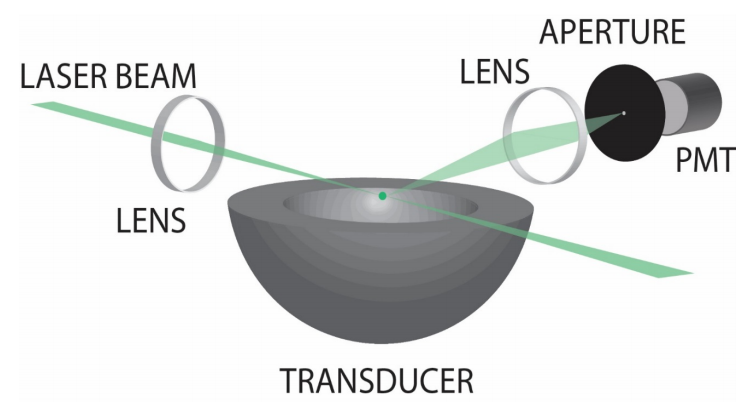
\includegraphics[width=100mm, height=50mm]{Nucleation_Experiment/experimental_setup.png}
\caption{A schematic showing working of the laser to detect nucleation. \cite{Yang2018}}
\label{laserSetup}
\end{figure}
\section{Results}
Figure \ref{probVoltage} shows the probability versus the voltage on the transducer. The two different thresholds are evident. Switching the voltage meant that the electrons from the radioactive source no longer reached the transducer. We know the nucleation events with the smaller threshold are from secondary electrons and the Penning ionization process. A low probability tail is observed in the curve. These events, with low threshold and low probability, are not explained by theory and are called very rare events.
\begin{figure}[H]
\centering 
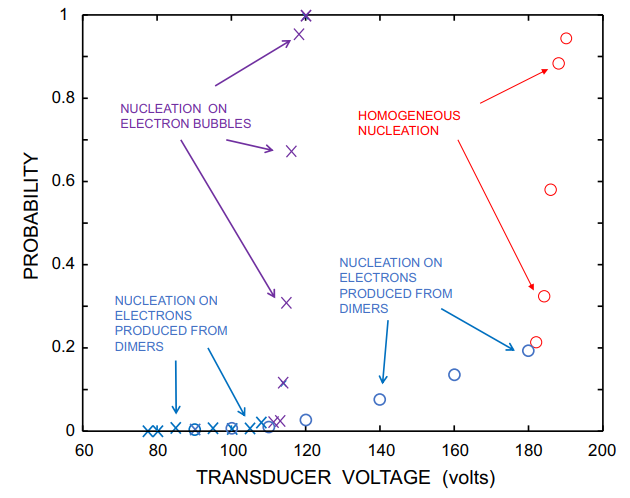
\includegraphics[width=100mm, height=80mm]{Nucleation_Experiment/probVsVoltage.png}
\caption{Probability of nucleation versus the voltage on transducer at $2.5$ K temperature and $0.42$ bar static pressure. The crosses represent data taken with $-200$ V on the source and the circles represent data with $+200V$ on the source. \cite{Yang2018}}
\label{probVoltage}
\end{figure}

It is possible that the rare events and very rare events are a result of nucleation of dust in the cell. Yang et all \cite{Yang2018thesis} conducted a separate experiment with a tip that was coated with carbon nanotubes as an electron source and produced the same results. Thus the rare events and very rare events are indeed related to electrons.

In order to study the rare events more carefully, we conducted experiments with a Thallium source. This is done because the number density of electrons is smaller for a Thallium source. Therefore the probability increases gradually with transducer voltage and we can study the rare events and very rare events carefully. Figure \ref{probVoltageThallium} shows the results with the Thallium source. It is clear that rare events are different than very rare events.
\begin{figure}[H]
\centering 
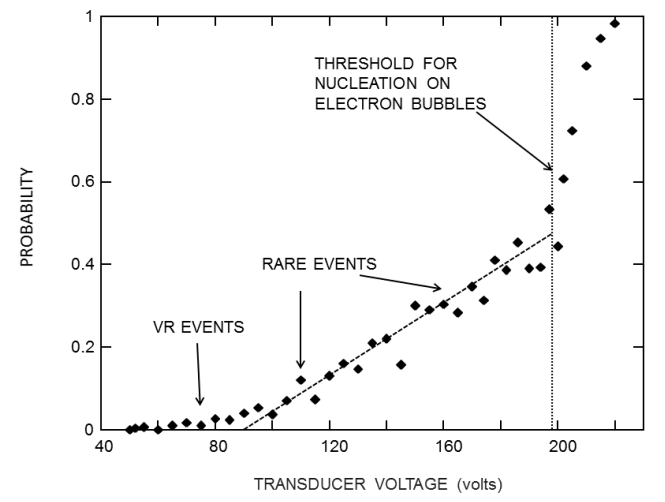
\includegraphics[width=100mm, height=80mm]{Nucleation_Experiment/thalliumSource.png}
\caption{Results using Thallium source \cite{Yang2018thesis}. The dashed line shows the threshold for caviation of electron the source. The data was taken at $3.00$ K temperature and $0.34$ bar static pressure.}
\label{probVoltageThallium}
\end{figure}
Below a certain voltage, the electrons from the source will not cavitate and the rare events will manifest in the probability voltage plot. The secondary electrons and penning ionization provide an explanation for rare events; however, not much is known about the very rare events.
\section{Deviation from prediction}
It was investigated how the threshold voltage discussed in the previous section varies with different temperatures and static pressures. The transducer was in thickness mode. As seen in Fig. \ref{non_linear1}, the variation against static pressure at a constant temperature is linear.
\begin{figure}[H]
\centering 
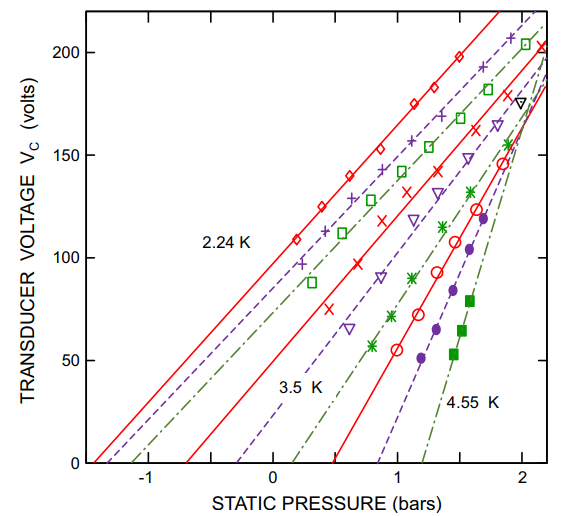
\includegraphics[width=100mm, height=80mm]{Nucleation_Experiment/non_linear1.PNG}
\caption{Threshold voltages for electron bubbles against static pressure for different temperatures. \cite{Yang2018thesis}}
\label{non_linear1}
\end{figure}

Thus the threshold voltage, $V_c$ can be written as
\begin{equation}\label{threshVoltageEq}
V_c=aP_{stat}+b
\end{equation}
Setting $V_c=0$, we can find the critical pressure $P_{el}$. This pressure is the static pressure which alone can produce cavitation in electron bubbles without the transducer. By linear fitting the data, we found the $P_{el}$ for different temperatures. The result is shown in Fig. \ref{non_linear2}. For comparison, we have also shown the data taken by Classen et al. \cite{Classen}
\begin{figure}[H]
\centering 
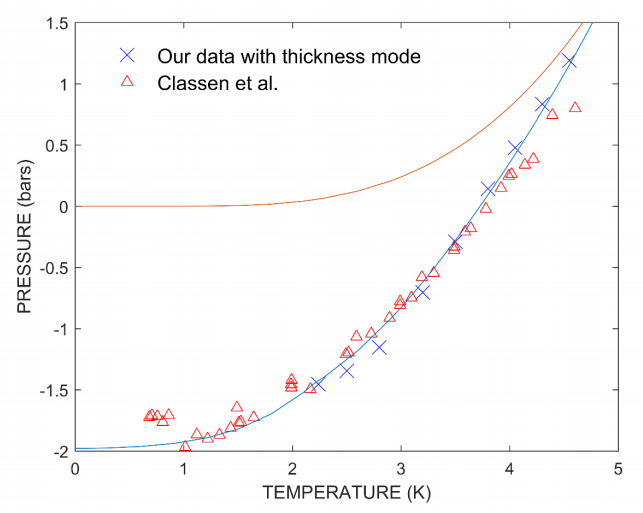
\includegraphics[width=100mm, height=80mm]{Nucleation_Experiment/non_linear2.png}
\caption{Critical pressure for nucleation versus temperature. The blue curve is the theoretical prediction by Eq. \ref{critPresseq}. The triangle points are from Classen et al. \cite{Classen} The yellow solid curve shows the saturated vapor pressure. \cite{Classen} \cite{Yang2018thesis}}
\label{non_linear2}
\end{figure}

Experimental data seems to agree quite well with that taken by Classen et al \cite{Classen} and the theoretical prediction for temperatures greater than $1$ K. Below $1$ K, they seem to be diverging from the expected value. Classen et al \cite{Classen} did not observe this since they did not collect data around $1$ K. It was also noted that the critical pressures measured with the flexural mode was always less negative than one with the thickness mode. One possible explanation is the sound waves in liquid helium have a nonlinear propagation. The sound might be getting distorted as it propagates due to nonlinearities in Helium. This would mean that the pressure at the focus might not be the same as the pressure at which we drive the transducer. This would especially be more prominent as the amplitude increases. We explore this possibility using simulations in the next chapter.

\chapter{Nonlinear correction}
\section{Motivation}
It was noticed that the critical pressure and temperature plot for cavitation of electron bubbles in liquid helium deviated from theoretical predictions at low temperatures in thickness mode. Nonlinear propagation of sound might be able to explain these experimental anomalies. The experimental data also suggests that if a linear fit were to be made, a certain static pressure alone is enough to produce the required negative pressure at the focus. This cannot be possible since, in the absence of driving, the pressure at the focus should be equal to the static pressure. The extrapolation gave a different pressure suggesting that some nonlinear calculations must be done in order to find the correct critical pressure for the bubble to burst.

We investigate whether the nonlinear propagation of the sound can be modeled using simulations and whether we can calculate the pressure at the focus due to the sound wave. To do this, we ran simulations to estimate the nonlinearity at two different frequencies, thickness mode (high frequency) and flexure mode (low frequency). We would like to know whether the relationship between the threshold voltage and the static pressure is nonlinear.

Understanding the propagation of sound in liquid helium will be crucial in future experiments concerning exotic ions since the exact pressure at the focus on the transducer needs to be known. We also need to know the consequences of using thickness mode for experiments.

\section{Background}

B.M. Abraham et al. proposed a Taylor series expansion of pressure: \cite{PhysRevA.2.550.3}

\begin{equation}\label{preseq1}
P = (\rho - \rho_0) \left.\frac{\partial P}{\partial \rho}\right|_0 + \frac{1}{2}(\rho - \rho_0)^2 \left.\frac{\partial^2 P}{\partial \rho^2}\right|_0 + \frac{1}{6}(\rho - \rho_0)^3 \left.\frac{\partial^3 P}{\partial \rho^3}\right|_0 + ...
\end{equation}

and found that\\

$\left.\frac{\partial P}{\partial \rho}\right|_0$ = c$_0^2$, $\left.\frac{\partial^2 P}{\partial \rho^2}\right|_0$ = $\frac{2c_0^2\mu_0}{\rho_0}$ and $\left.\frac{\partial^3 P}{\partial \rho^3}\right|_0$ = $\frac{2c_0^2\mu_0}{\rho_0}$ + $\frac{2c_0^2w_0}{\rho_0}$\\

The constants $\rho_0$ and $c_0$ are the density and sound velocity at zero pressure, respectively. The constant $\mu_0$ is known as the Gruneisen Constant. B.M. Abraham et al \cite{PhysRevA.2.550.3} found the Gruneisen Constant in liquid helium to be $2.84$. The experiment was made in the vicinity of $0.5$ K. They also found that $w_0$, another experimental constant, is $0.194$.

This Taylor series expansion can be used to simulate the propagation of sound in liquid helium. We will consider the first three terms in our calculations. In the simulations, the traducer wall was driven as:

\begin{equation}\label{diseq}
u_t = u_0 sin(\omega t)(1-e^{\frac{-t}{\tau}})
\end{equation}
Where $u_0$ is the initial displacement of the wall and $u_t$ is the displacement at time $t$. $u_0$ is proportional to the voltage applied to the transducer. $\tau$ is the time needed for the transducer amplitude to build up. The equation models the build up of sound well because we require the amplitude of the pressure to increase linearly for a short time. This can be achieved by Eq. \ref{diseq} since from the first order Taylor series expansion of $e^{\frac{-t}{\tau}}$, for small t:
$$1-e^{\frac{-t}{\tau}} \approx 1 - 1 + \frac{-t}{\tau}  \approx \frac{-t}{\tau}$$
This means that at the peaks, where $sin(\omega t)$ is equal to $1$, the amplitude should increase linearly. For larger times, the exponential term will die out and the oscillations would be sinusoidal. Finally, differentiating Eq. \ref{diseq} with respect to time would yield the velocity. 

\section{Simulation Algorithm}
First, an array with various values of $r$, the number of which depend on the impute parameters, is created from $r = 0$ to $r = 0.8$ cm (which is the distance of focus from the transducer). As the program loops through the time, each value of $r$ is assigned a corresponding density which is given by the following relations:

\begin{equation}\label{radeq1}
Vol_{intl} = \frac{4}{3}\pi [(r_{n+1})^3 - (r_n)^3]
\end{equation}

\begin{equation}\label{radeq2}
Vol_r = \frac{4}{3}\pi [(r_{n+1} + u_{t+1})^3 - (r_n + u_t)^3]
\end{equation}

\begin{equation}\label{deneq1}
\rho_r = \rho_{intl} \frac{Vol_{intl}}{Vol_r}
\end{equation}

$Vol_{intl}$ is the initial volume between $r = r_n$ and $r_{n+1}$.Thus the $nth$ value of $Vol_{intl}$ is the volume of the shell between the $(n+1)th$ value of $r$ and $(n+1)th$ value of $r$. Similarly, $Vol_n$ is volume of the shell between the $nth$ value of $r$ and $(n+1)th$ value of $r$ when the sound wave is going through the liquid. $\rho_{intl}$ is the density of helium at a given static pressure. Therefore being constant throughout the experiment. Due to the propagation of the sound wave, the displacement of the wave at a given point must be added to the corresponding value of $r$ in order to find the correct value of $Vol_r$. The instantaneous density of the liquid $\rho_r$, at radius $r$, is calculated using Eq. \ref{deneq1}. Finally, the corresponding pressure $P$, at radius $r$ and time $t$, is calculated from $\rho_r$ using Eq. \ref{preseq1} setting $\rho$ = $\rho_r$.

\section{Results}

The pressure at the focus was plotted against time in Fig. \ref{presvstime} for both resonant frequencies. The static pressure in each case was $1.0$ atm. The initial straight line, indicating the time sound needs to reach the focus, agrees with what one would expect using the velocity of sound in liquid helium and the radius of focus.
\begin{figure}[H]
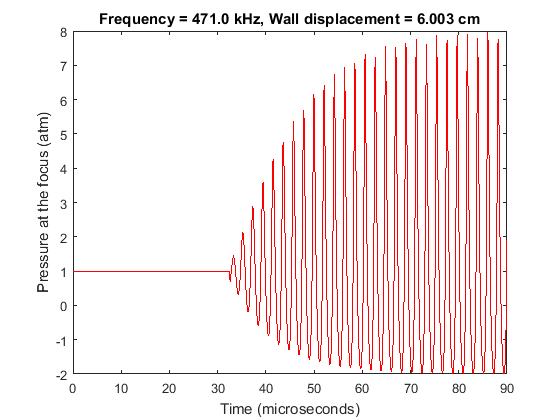
\includegraphics[width=75mm, height=60mm]{Nonlinear_correction/pvt_hf.png}
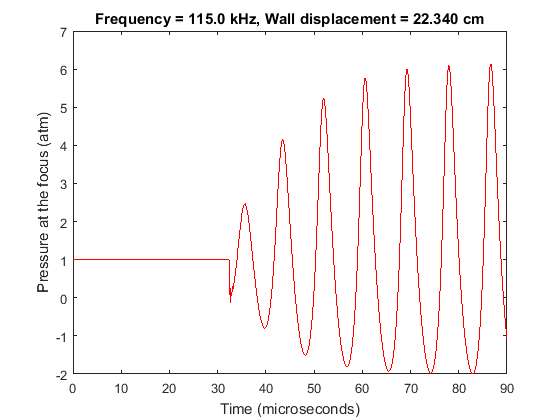
\includegraphics[width=75mm, height=60mm]{Nonlinear_correction/pvt_lf.png}
\caption{Pressure versus Time plots for the focus.}
\label{presvstime}
\end{figure}
Figure \ref{presvsrad} shows the pressure vs radius plot. $r=0$ corresponds to the focus. The static pressure was $1.0$ atm. The plot shows that pressure at focus (where $r=0$) is the maximum. The transducer is hemispherical. Therefore, the focus is equidistant from all point on the transducer. Thus the sound waves convergence at the focus interfering constructively. This is because they all have the same phase.
\begin{figure}[H]
\centering 
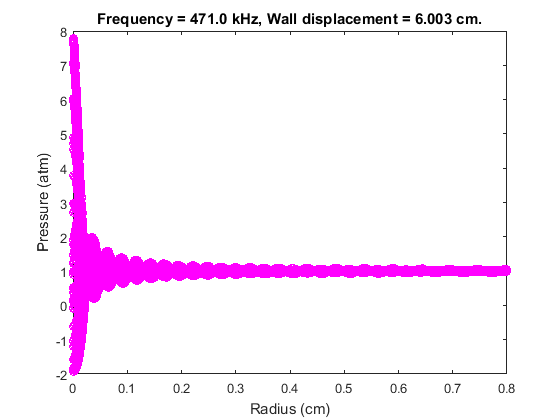
\includegraphics[width=75mm, height=60mm]{Nonlinear_correction/prevsrad.png}
\caption{Pressure versus time plots for the focus.}
\label{presvsrad}
\end{figure}

Ultimately, the goal was to find the displacement of the wall that gives a pressure of -2 atm at the focus. This was done by varying the initial amplitude of the wall, keeping the static pressure constant. The initial density for a given static pressure was found by solving Eq. \ref{preseq1} for $\rho$. A plot of displacement of the wall versus static pressure is shown in Fig. \ref{disvspress}. The third plot in Fig. \ref{disvspress} shows the same relations, but with minimum pressure at the focus being $-1$ atm.

\begin{figure}[H]
\begin{tabular}{cc}
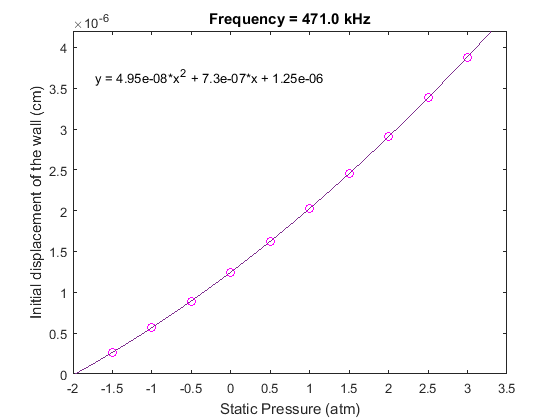
\includegraphics[width=75mm, height=60mm]{Nonlinear_correction/p_-2_hf.png} 
& 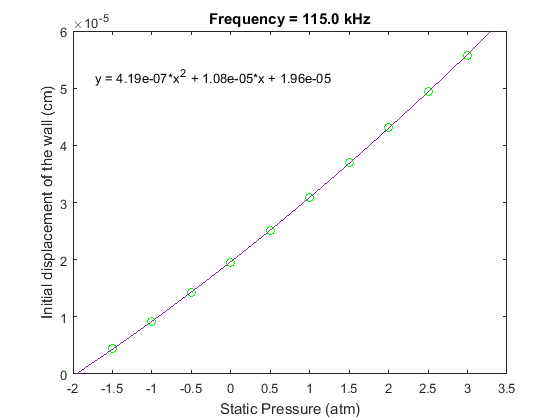
\includegraphics[width=75mm, height=60mm]{Nonlinear_correction/p_-2_lf.png}\\
\multicolumn{2}{c}{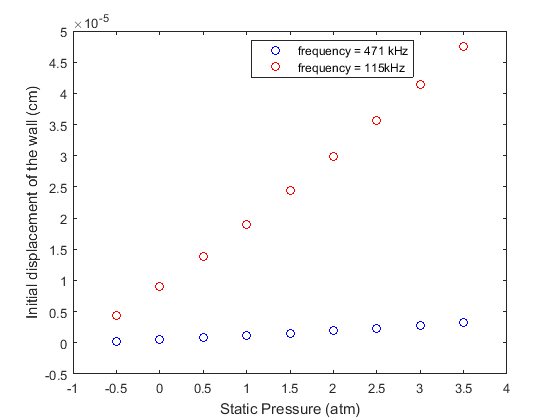
\includegraphics[width=75mm, height=60mm]{Nonlinear_correction/p-minus1.png}}\\
\end{tabular}
\caption{Displacement versus static pressure plots.}
\label{disvspress}
\end{figure}

The plot of displacement verses static pressure was found to be non linear. This means that the nonlinear propagation of sound must have impacted the pressure-temperature plot in Chapter 2. It was also observed that the nonlinear effects were more prominent at high frequency. This also agrees with the experiment since the anomalies were found to be significant at high frequency. The displacement versus pressure relations can used for calculations. A quadratic linear fit has been included in Fig. \ref{disvspress}. Ideally the curve should have passed through $(-2,0)$ and $(-1,0)$ for a static pressure of $-2$ atm and $-1$ atm respectively; however, the fit came really close to those points. 

Thus the simulation was quite successful in modeling the propagation of sound waves in the liquid. The most basic requirement was that the pressure at the focus should be higher than any point in the liquid. It was also expected that the amplitude of the pressure should increase linearly for a short time. Both of these requirements were satisfied. We also concluded that the propagation of sound in liquid helium is indeed nonlinear. This type of calculation can form a basis for future experiments involving exotic ions.



\chapter{Conclusion}
\section{Summary and discussion}

To conclude, electrons in liquid helium form an interesting quantum mechanical system and can be studied through experiments. The goal of experimenting with electrons was also to design future experiments for studying exotic ions. These electron bubbles can be cavitated by applying a certain negative pressure. We found that there are two different thresholds for cavitation in electron bubbles. Each has a different mechanism which was studied in detail. The experiments also suggested a new event called very rare event of which not much is known. While studying the variation of critical static pressure with temperature, we were motivated to perform calculations for non linear propagation of sound in liquid helium.

The calculations for propagation of sound were quite successful in modeling the system. All the basic requirements were met and we recorded the correct pressure oscillation. We saw that the relation between critical static pressure and temperature is indeed nonlinear. Thus this simulation would help in studying exotic ions in the future.


\section{Future directions}
In order to understand the structure and energy levels of these exotic ions, experiments involving quantized vortices can be performed. It is possible to trap exotic ions inside quantum vortices. \cite{Milliken1982} Once trapped, the exotic ion can be excited with a laser. \cite{DEGROOT1985445} Finding the critical wavelength- where the exotic ion barely escapes the vortex- would help in determining the energy levels of the exotic ion.

Recent experiments involving calculating the mobility of charged ions in liquid helium suggests the existence of positively charged ions in liquid helium. It is possible that these ions could be clusters of helium molecules around a positive helium ion. In order to see if that is possible, we ran molecular dynamics simulations. The formation of the cluster was identified using the coefficient of self-diffusion. If there is a cluster formed, the coefficient of the diffusion for atoms near the charged molecule should be much smaller than for molecules far from it. The ultimate goal is to start with a positively charged helium molecule and neutral helium molecule in a box. Then we would let them interact for a while and see if they clump together to form a cluster. Later we can attempt to model the structure of this cluster. Finally, we need to make sure that the simulation is modeling the system correctly and make detailed calculations involving diffusion coefficients.

It was concluded that it is difficult to investigate the displacement-static pressure relationship for the thickness mode by means of simulation. This is because the sound field produced by the thickness mode is very complex. It was found that the transducer vibrates in a complex manner when driven with high frequency. These vibrations cannot be represented by a single equation and thus more sophisticated simulations need to be performed. It is also possible that if the pressure swing is big enough, the numerical simulation might explode at the focus. This might be due to a shock formation. A possible solution is to use the WENO scheme. \cite{Appert2003}

\printbibliography
\end{document}
